%!TEX root = ../main.tex

\chapter{Tire Physical Modeling}
\label{app3:tirex}

We present a novel tire brush model with carcass flexibility, primarily designed for real-time applications while preserving the physical significance of its parameters. The model has been already presented in~\cite{stocco2024physical}, and it is here reported to provide a comprehensive overview of the tire modeling approach. Specifically, it is built upon the methodologies in~\cite{stocco2021acme,stocco2024novel}, also outlined in Appendix~\ref{app1:acme} and Appendix~\ref{app2:enve}. The tire's geometry is discretized and represented using a series of ribs, each intersecting the local road surface independently. The carcass in-plane fore-aft displacement, in-plane deflection, and out-of-plane sidewall torsion are approximated through a second-order polynomial. Forces and torques originating from the tire-road contact area are described using brush mechanics. Notably, the kinematics of the bristles are directly linked to carcass deformation. Extensive effort is dedicated to understanding the possible sources of instability, as well as describing and implementing a robust numerical scheme to effectively solve the non-linear system of equations arising from the modeling. Numerical performance results are provided to demonstrate the suitability of the presented model for demanding hard real-time simulations. Validation of the model here presented is carried out by fitting experimental data and comparing it with the state-of-the-art \MagicFormulae{} model, proving its reliability and accuracy in reproducing tire behavior.

% % % % % % % % % % % % % % % % % % % % % % % % % % % % % % % % % % % % % % % %

\section{Introduction to Tire Modeling}
\label{app3:sec:introduction}

Numerous investigations and experiments have been conducted over the past century to understand tire characteristics and behavior, revealing a close relationship between tire performance and the technologies, techniques, and materials used in manufacturing~\cite{nakajima2019advanced, gil2020inplane}. However, accurately modeling tire characteristics from construction specifications is challenging due to the complex tire internal structure. To tackle this challenge, two main modeling approaches have been proposed so far: \emph{empirical} and \emph{physical}~\cite{guiggiani2014science, rill2020road, pacejka2012tire, oertel2015years}.

The empirical approach is popular because of its simplicity, low computational cost, and ability to capture accurate tire behavior. In this approach, tire-road interaction forces are approximated using a combination of functions derived from physical insights, as well as years of experimental campaigns and experience. The identification process for computing the set of parameters that best fit experimental data for a specific tire is one of the biggest challenges for these models. The \MagicFormulae{} model, initially developed by~\citet{bakker1987tyre} and later improved multiple times~\cite{pacejka2012tire}, is the most-known and state-of-the-art empirical model. It fits experimental data through a sequence of numerical optimizations on predetermined curve shapes~\cite{bayle1993new}. Due to its diffusion, low computational complexity and overall performance, the \MagicFormulae{} model is considered the standard in both data fitting and vehicle simulation~\cite{guiggiani2014science, pacejka2012tire}.

The physical approach involves direct geometrical and physical tire modeling, providing a deeper understanding of the complex phenomena related to tire behavior~\cite{nakajima2019advanced}. While the computational burden heavily depends on the desired accuracy, this approach can better generalize behavior without fitting a large experimental dataset for every specific tire. Additionally, physical models usually depend on a smaller number of parameters that have a direct physical meaning. The \ac{FE} method represents a physical approach to tire modeling primarily used, though not exclusively, for assessing static characteristics, stiffnesses, resonant frequencies, and vibration modes~\cite{taheri2014technical}. Another physical modeling technique is based on the \ac{DE} method~\cite{karpman2020discrete}, which employs a limited number of interconnected elements and nodes to mimic the degrees of freedom and constraints of real tire carcass structures~\cite{gipser2005ftire, gallrein2007cdtire, yamashita2016physicsbased}. Prominent \ac{DE} models like \FTire{} and \CDTire{} are capable of running under real-time environments~\cite{cosinscientific, gallrein2014advanced}, and encompass advanced features such as detailed external geometry description, flexible and visco-plastic rim, air cavity vibration, deformable and visco-elastic ground soil compatibility, as well as temperature and wear modeling. However, the availability of detailed information regarding the computational time performance of both \FTire{} and \CDTire{} remains limited.

A big branch of physical modeling relies on the brush mechanics theory~\cite{pacejka2012tire}, which originates from a simplified version of Kalker's conformal contact theory~\cite{kalker1967rolling, kalker1971transient, kalker1979survey, kalker1986railway, kalker1997simulation, meymand2016survey}. This theory assumes the road surface to be non-deformable, and describes the tire behavior within the contact patch area using one or more rows of radial bristles along or parallels to its equator, having a frictional constraint with the road, and deflecting according to kinematic equations. Over the years, several extensions of the original brush model have emerged, addressing dynamic friction behavior~\cite{deur2004brush, deur2005extensions, velenis2005dynamic, kikuuwe2019brushtype}, realistic contact pressure distribution~\cite{miyashita2010tire, fevrier2013method, xu2014analytical}, high camber angles and high steering speeds~\cite{higuchi1999transient, romano2022analytical}, carcass deformation influence~\cite{svendenius2006semiempirical, xu2014analytical, miyashita2010tire, miyashita2003analytical, miyashita2006new, kabe2006new, miyashita2015study, romano2019novel, romano2020unsteadystate, gil2020inplane}, effects of temperature and wear~\cite{fevrier2013method, harsh2019tire}, and a more accurate description of external tire morphology~\cite{chollet2012model, riehm2019brush}. Brush models are effective at efficiently capturing the behavior of the tire tread layer, and they can also be coupled to a simplified carcass deformation model under proper assumptions. Sakai's~\cite{sakai1981theoreticalI, sakai1981theoreticalII, sakai1981theoreticalIII, sakai1982theoreticalIV}, \NeoFiala{}~\cite{miyashita2003analytical, miyashita2006new, kabe2006new, miyashita2015study, miyashita2010tire}, \TreadSim{}~\cite{dehoogh2005implementing}, and \TaMeTire{}~\cite{fevrier2013method} are three notable advanced tire models that combine a brush model with a carcass deflection and, although different in design, they can accurately describe significant tire characteristics that are beyond the capabilities of empirical models. These include: (1) advanced frictional properties at the tire-road interface, such as local contact pressure and velocity dependency of the friction coefficient; (2) description of the tangential stress within the contact patch, crucial for understanding the tire's lateral and longitudinal force generation; and (3) carcass in-plane fore-aft displacement and deflection, and out-of-plane sidewall torsion, often described through a beam on elastic foundation or a second-order polynomial approximation.

Despite the extensive literature on tire modeling, the author aims to develop a novel tire model suitable for real-time vehicle simulations, highlighting the scope for further enhancement in the field of tire modeling. This new model is built upon a minimal set of physical parameters rather than empirical formulas, to characterize tire properties. For this reason, the contributions of this thesis to the existing state-of-the-art tire modeling include the development of a fully scalable physical tire model capable of running within a time step of \SI{1}{\milli\second}. Such a time step is a typical requirement for real-time simulations that aim at reproducing stiff subsystems with high-frequency dynamics~\cite{pacejka2012tire}. The tire model is structured modularly, facilitating straightforward extension to incorporate additional features such as the effect of temperature and wear, and not less importantly, to achieve the desired computational performance through the newly developed numerical solution scheme. Possible sources of instability are also analyzed, and practical solutions to ensure robustness are discussed. In summary, this study aims to advance the current understanding of flexible carcass tire model behavior and provide a numerical framework enabling the newly developed physical tire model's integration into hard real-time simulations. To demonstrate the suitability of the proposed model in such demanding conditions, timing and numerical scheme performance outcomes are provided. Validation of the model is performed by fitting experimental data provided by the \ac{TIRF} for the \ac{FSAE} \ac{TTC} testing program (refer to \citet{kasprzak2006formula} for a comprehensive description \ac{FSAE} \ac{TTC}'s testing set-up, procedures, and data acquisition), as well as by comparing it with the state-of-the-art \MagicFormulae{} model, ensuring its reliability and accuracy in reproducing tire behavior.

% % % % % % % % % % % % % % % % % % % % % % % % % % % % % % % % % % % % % % % %

\section{Tire Modeling}
\label{app3:sec:tire_modeling}

Pneumatic radial tires are inflated composite structures whose primary structural subcomponents are the \emph{rim}, the \emph{carcass}, and the \emph{tread}. While the rim maintains tire shape, the carcass constitutes the main tire structure connecting the rim to the tread. The tread, on the other hand, serves as the outer rubber layer providing a link between the road and the carcass. In the following sections, we will describe the tire modeling approach, focusing on the carcass and tread, as the rim is considered a rigid body.

\subsection{Tire and Road Geometric Representation}
\label{app3:sec:tire_road_representation}

Let us consider a reference frame $\pt{H}xyz$ with unit vectors ($\et{h}_x$, $\et{h}_y$, $\et{h}_z$),  having its origin $\pt{H}$ located at the wheel hub. The axes are oriented according to the ISO 8855:2011 standard~\cite{iso88552011}. The $x$-axis is directed towards the longitudinal direction of motion, the $z$-axis points upward, and the $y$-axis is oriented so that the coordinate system is right-handed (refer to \figurename~\ref{app3:fig:tire_iso}).  Geometrically, the tire is characterized as axially symmetric (about the axis $\et{h}_y$), convex, and closed set $\sett{T}$ defined as
%
\begin{equation*}
  \sett{T} = \left\{ \begin{bmatrix} x\\ y\\ z \end{bmatrix} \in \mathbb{R}^3, ~ y \in \left[ y_l, y_r \right], ~ R(y):\mathbb{R} \mapsto \mathbb{R} ~\big|~ \sqrt{x^2+z^2} \leq R(y) \right\} \, \text{.}
\end{equation*}
%
Here, the function $R(y)$ can be chosen arbitrarily to reconstruct the desired outermost shape of the tire. On the other hand, the road is modeled as a closed half-space $\sett{R}$ whose boundary is defined by the plane passing through the point $\pt{p}$ with unit normal $\et{n}$, \ie{},
%
\begin{equation*}
  \sett{R} = \left\{\undx{}\in\mathbb{R}^3 ~|~ (\undx{}-\pt{p})\cdot\et{n} \leq 0 \right\} \, \text{,}
\end{equation*}
%
where $\undx{} = [x,y,z]^\top$. The contact patch region is defined as a closed set $\sett{P}$ comprising all the points of the tire $\sett{T}$ which are also interior points of the road boundary surface $\boundary{R}$, \ie{}, $\sett{P} = \sett{T} \cap \boundary{R}$. The contact patch reference frame $\pt{O}xyz$ has the origin in $\pt{O}$, which corresponds to the centroid of the region $\sett{P}$. Its unit vectors ($\et{e}_x$, $\et{e}_y$, $\et{e}_z$) are defined as $\et{e}_x = \et{h}_x$, $\et{e}_y = \et{n} \times \et{e}_x$, and $\et{e}_z = \et{n}$.

\begin{figure}[htb]
  \centering
  \begin{minipage}[t]{0.425\linewidth}
    \centering
    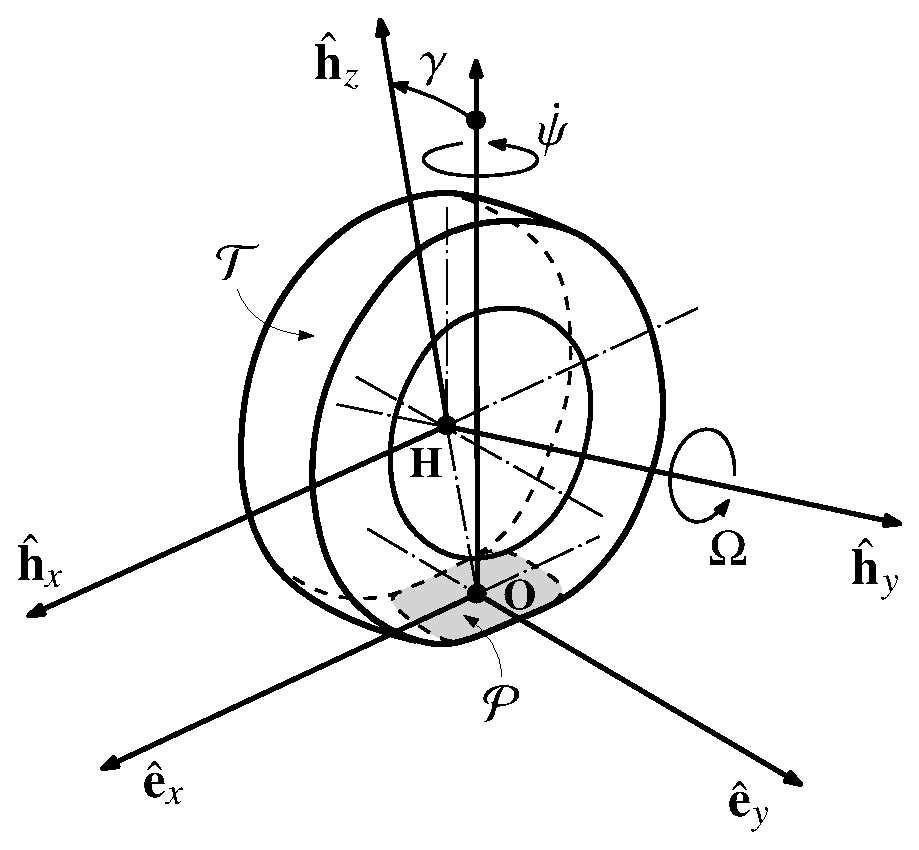
\includegraphics[width=0.9\linewidth]{figures/appendix_3/tire_iso}
    \caption{Tire-road schematics according to ISO coordinate system~\cite{iso88552011}.}
    \label{app3:fig:tire_iso}
  \end{minipage}
  \hfill
  \begin{minipage}[t]{0.525\linewidth}
    \centering
    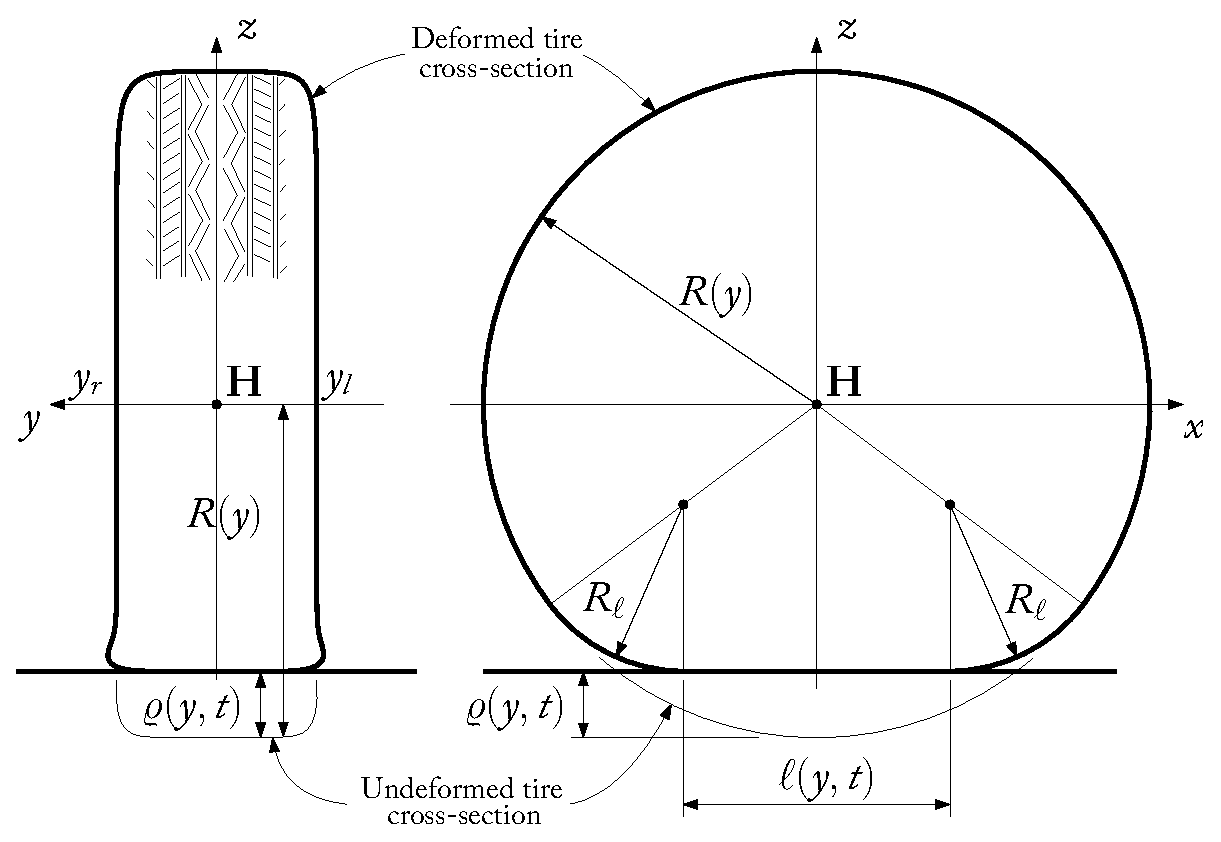
\includegraphics[width=1.0\linewidth]{figures/appendix_3/belt_section}
    \caption{Illustration of the tire-road contact geometry parameters.}
    \label{app3:fig:belt_section}
  \end{minipage}
\end{figure}

% % % % % % % % % % % % % % % % % % % % % % % % % % % % % % % % % % % % % % % %

\subsection{Tire-Road Vertical Contact Mechanics}
\label{app3:sec:vertical_contact}

When the contact patch set is not empty (\ie{}, $\sett{P} \neq \varnothing$) there is a multitude of contact points $\undx{} = [x,y,z]^\top \in \sett{P}$. At each point, the stress component along the $z$-axis (also known as normal stress) $q_z(\undx{},t)$ is applied. The integral of the normal stress distribution over the entire contact patch region is equal to the tire's vertical load $F_z(t)$. The vertical normal stress distribution is extremely difficult to calculate analytically, and it depends on the tread pattern properties, carcass stiffness, friction and inflation pressure~\cite{nakajima2019advanced}. To easily model the tire's vertical characteristics, we employ a single-contact point approach. The total vertical tire stiffness is calculated as
%
\begin{equation*}
  k_z(\omega, \gamma, p) = k_z^s + k_z^p p + k_z^\omega \omega + k_z^\gamma \gamma^2 \, \text{.}
\end{equation*}
%
Here, $k_z^s$ represents the structural vertical stiffness, $k_z^p$ denotes the vertical stiffness dependence on inflation pressure, $k_z^\omega$ indicates the vertical stiffness dependence on rolling speed, and $k_z^\gamma$ is the vertical stiffness dependence on camber angle. The total vertical force is thereby calculated as
%
\begin{equation}
  F_z(t) = k_z(\omega(t), \gamma(t), p) \rho(t) + c_z \dot{\rho}(t) + k_z^b \max(0, \rho(t)-\rho_b) \, \text{,}
  \label{app3:eq:vertical_force}
\end{equation}
%
where $F_z \in \mathbb{R}_{\geq 0}$, $\rho(t) \in \mathbb{R}_{\geq 0}$ represents the deflection at the tire contact point, $\rho_b$ represents the bottoming threshold, $c_z$ is the vertical damping coefficient, and $k_z^b$ indicates the bottoming vertical stiffness. Specifically, the tire contact point deflection $\rho(t)$ is calculated with the method outlined in~\cite{stocco2024novel, stocco2021acme}. This technique not only facilitates efficient and robust computation of the contact point deflection $\rho(t)$ but also allows us to compute the tire deflection $\varrho(y,t)$ at a specific lateral coordinate $y$ and time $t$. Alternatively, for cases where the technique outlined in~\cite{stocco2024novel} is not employed, a viable approximation, particularly for small camber angles ($|\gamma(t)| < \pi/10$), is
%
\begin{equation*}
  \rho(t) = \max_{y \, \in \, [y_l, y_r]} \varrho(y,t) \qquad \text{(refer to \figurename~\ref{app3:fig:belt_section})} \, \text{.}
\end{equation*}

\subsubsection{Contact Patch Length}
\label{app3:sec:contact_patch}

The geometrical intersection between the tire set $\sett{T}$ and road boundary surface $\boundary{R}$ provides us only a rough approximation of the tire-road contact patch area. Based on the findings in~\cite{koutny2007geometry, rhyne2005development}, we introduce a contact transition radius $R_\ell \in \mathbb{R}_{\geq 0}$ to take the tire belt stiffness into account and get a more realistic result (see \figurename~\ref{app3:fig:belt_section}). The contact length at any given lateral coordinate $y$ on the contact patch reference system can be computed as
%
\begin{equation}
  \ell(y,t) = 2\sqrt{\big(2(R(y)-R_\ell) - \varrho(y,t)\big)\varrho(y,t)} \, \text{,}
  \label{app3:eq:contact_length}
\end{equation}
%
where $\varrho(y,t)$ is the tire radial deflection. Notice that the equation~\eqref{app3:eq:contact_length} can be easily found from the study of \citet{rhyne2005development} by imposing null radial counter-deflection.

\subsubsection{Contact Pressure Distribution}
\label{app3:sec:pressure_distribution}

The pressure distribution is one of the most complex, challenging-to-model factors significantly impacting tire behavior~\cite{savkoor1966some}. Both experimental results and \ac{FE} analyses reveal that the pressure trend over the contact patch is strongly three-dimensional and is influenced by numerous factors, including carcass structural stiffness, contact pressure, relative camber angle, tread pattern topology, and local road macro-roughness. Experimental evidence suggests that adequately inflated modern radial tires typically exhibit a plateau in the pressure distribution at the central part of the contact patch~\cite[Chapter~5]{nakajima2019advanced}. Conversely, overinflated and underinflated radial tires may have more complicated distribution shapes~\cite{nakajima2019advanced, sakai1995measurement}. Recent efforts have been aimed at more detailed modeling of the contact patch to better match experimental results~\cite{miyashita2010tire, fevrier2013method, xu2014analytical}. An interesting approach involves modeling the contact pressure distribution using a quartic polynomial function $\Upsilon(\chi) = c_0 + c_1\chi^1 + c_2\chi^2 + c_3\chi^3 + c_4\chi^4$. This function represents the normalized contact pressure distribution shape along the normalized longitudinal coordinate $\chi \in [0, 1]$. To determinate the polynomial coefficients $c_0, \dots, c_4$ the following constraints are imposed
%
\begin{equation}
  \begin{cases}
    \dfrac{\mathrm{d}^2}{\mathrm{d}\chi^2}\Upsilon\left(\dfrac{1}{2}\right) = -\lambda & \text{convexity at the center of the contact patch $\chi = \dfrac{1}{2}$,}
    \\[1.0em]
    \displaystyle\int_{0}^{1} \Upsilon(\chi)\,\mathrm{d}\chi = 1 & \text{normalization condition for the total contact force over the contact patch,}
    \\[1.0em]
    \displaystyle\int_{0}^{1} \Upsilon(\chi)\chi\,\mathrm{d}\chi = \dfrac{1}{2} - \delta & \text{barycentre shift with respect to the center of the contact patch $\chi = \dfrac{1}{2}$,}
    \\[1.5em]
    \Upsilon(0) = \Upsilon(-1) = 0 & \text{absence of pressure at the edges of the contact patch $\chi = 0$ and $\chi = 1$.}
    \\[0.5em]
  \end{cases}
  \label{app3:eq:upsilon}
\end{equation}
%
Then, we solve for $c_0, \dots, c_4$, and the solution of the system is
%
\begin{equation*}
  c_0 = 0, \quad
  c_1 = -\dfrac{1}{3}\lambda + 10 + 60\delta \, \text{,} \quad
  c_2 = 2\lambda - 30 - 180\delta \, \text{,} \quad
  c_3 = -\dfrac{10}{3}\lambda + 40 + 120\delta \, \text{,} \quad \text{and} \quad
  c_4 = \dfrac{5}{3}\lambda - 20 \, \text{.}
\end{equation*}
%
Here, $\lambda \in \mathbb{R}$ and $\delta \in \mathbb{R}$ respectively denote the convexity and longitudinal barycentre shift of the base curve $\Upsilon(\chi)$. The only drawback of this approach is that for certain values of $\delta$ and $\lambda$, the condition of positive pressure $\Upsilon(\chi) \ge 0$ within the range $\chi \in [0,1]$ is not always guaranteed and must be numerically checked in the software implementation. Thus, a careful selection of these parameters is essential. On the other hand, the use of a polynomial to describe the pressure distribution over the contact patch allows us to adopt some numerically robust algorithms and efficient evaluations for some of the calculations that will follow. Given the objective of achieving real-time applicability for the numerical tire model, this aspect should not be overlooked. The vertical contact stress distribution $q_z(\undx{},t)$ is then written as
%
\begin{equation}
  q_z(\undx{},t) = \dfrac{F_z(t)}{A_\sett{P}(t)}\Upsilon\left(\dfrac{\ell(y,t)/2-x}{\ell(y,t)}\right) \, \text{,} \\
  \label{app3:eq:vertical_stress}
\end{equation}
%
where $\undx{} = [x,y,z]^\top \in \sett{P}$, $F_z$ denotes the tire's vertical load, and $A_\sett{P}$ represents the contact patch area, defined as
%
\begin{equation*}
  A_\sett{P}(t) = \displaystyle\int_{y_r}^{y_l} \ell(y,t)\,\mathrm{d}y \, \text{.}
\end{equation*}
%
It must be stressed that the contact patch region $\sett{P}$ is a function of time $t$ and of the lateral coordinate $y$. This variability arises because the contact patch is not fixed but rather a function of the tire-road contact geometry.

% % % % % % % % % % % % % % % % % % % % % % % % % % % % % % % % % % % % % % % %

\subsection{Tire-road Tangential Contact Mechanics}
\label{app3:sec:tangential_contact}

In the present work, we assume that the vertical problem can be decoupled from the tangential, implying that the tangential stresses do not affect the vertical one, but not vice versa. Additionally, the vertical and lateral carcass flexibility characteristics are assumed to be fully independent. In simpler terms, we assume that neither friction-related phenomena nor carcass deformation affect the vertical pressure distribution $q_z$. Consequently, we can analyze tire-road tangential contact mechanics sequentially from the vertical component, while still maintaining the tangential contact forces proportionality to the vertical load $F_z$. It is worth noting that this assumption greatly simplifies the numerical solution of the tire model, as it avoids the need to find the vertical and tangential forces through a system of nonlinear equations, which would be computationally expensive.

% % % % % % % % % % % % % % % % % % % % % % % % % % % % % % % % % % % % % % % %

\subsubsection{Carcass Deformation Model}
\label{app3:sec:carcass_model}

In numerous tire models, the carcass is modeled as a beam on elastic foundation~\cite{dehoogh2005implementing, sarkisov2019physical, gil2020inplane, nakajima2019advanced}. Experimental findings from the studies~\cite{sarkisov2019physical, gil2020inplane} demonstrate that carcass deflection comprises both bending and shears components. The significance of the shear contribution varies depending on the carcass ply cord angles. Consequently, formulations like the Timoshenko-Ehrenfest or Euler-Bernoulli beam are particularly suited to describe the lateral bending of carcass structure in the cornering conditions~\cite{gil2020inplane}. Models like those in~\cite{fiala1954seitenkraften, miyashita2006new, kabe2006new, xu2014analytical, gil2020inplane, sakai1981theoreticalI, sakai1981theoreticalII, sakai1981theoreticalIII, sakai1982theoreticalIV, miyashita2010tire, fevrier2013method} adopt a second-order polynomial (parabola) as a local approximation of the beam on elastic foundation in the proximity of contact patch area. This approach provides a straightforward yet accurate description of the deformed carcass centreline within the contact region. However, the models currently present in the literature are only able to fully describe the lateral deformation and do not allow for modeling the longitudinal displacement. Indeed, during traction, braking and cornering, the contact patch is subject to non-negligible fore-aft, lateral, bending and torsional displacements. These displacements strongly impact the generation of longitudinal, lateral, and vertical forces, as well as rolling resistance, overturning, and self-alignment torques. To take into account the longitudinal displacement of the carcass, we define the two-dimensional carcass centreline as
%
\begin{equation}
  \sett{L}(\undx{}, \vt{c}) =
  \begin{bmatrix}
    \sett{L}_x \\[0.2em]
    \sett{L}_y
  \end{bmatrix} =
  \begin{bmatrix}
    x_c \\[0.2em]
    y_c + \theta_c(x-x_c) - y_c\dfrac{\Psi}{2}(x-x_c)^2
  \end{bmatrix} \, \text{,}
  \label{app3:eq:parabola}
\end{equation}
%
where time-dependent parameters $x_c$ and $y_c$ represent the carcass longitudinal and the lateral translating deformations, respectively, $\theta_c$ denotes the carcass twisting angle, and $\Psi$ is the lateral bending shape factor. As depicted in \figurename~\ref{app3:fig:contact_patch}, we model the carcass deformation through a point $\vt{c} = [x_c, y_c, \theta_c]^\top$ described within the contact patch reference frame $\pt{O}xyz$. The carcass point $\pt{c}$ is connected through a set of independent spring elements to the point $\left[0, 0, -R_z\right]^\top$, defined in the hub reference frame $\pt{H}xyz$, where $R_z = \et{n} \cdot (\pt{H}-\pt{O})$.

\begin{figure}[htb]
  \centering
  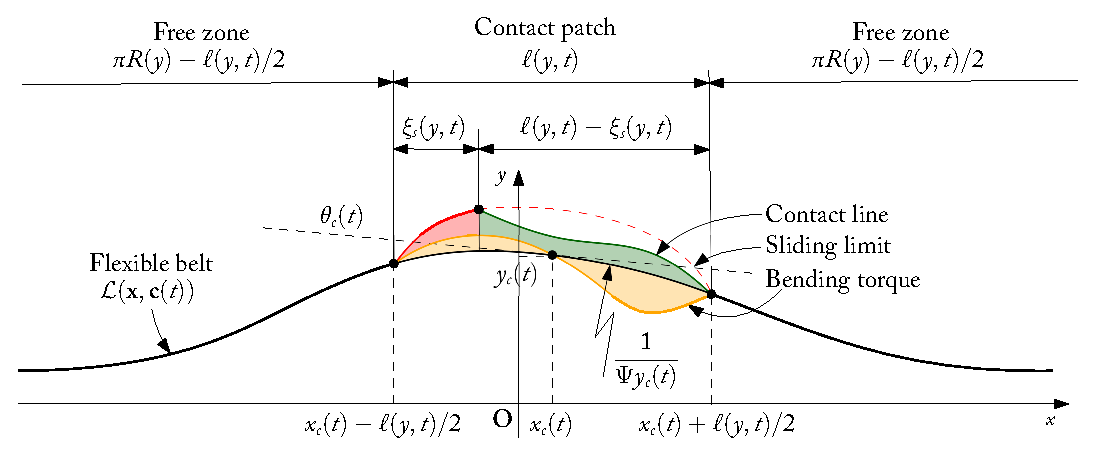
\includegraphics[width=0.8\linewidth]{figures/appendix_3/contact_patch}
  \caption{Depictions of the deformed carcass baseline $\sett{L}(\undx{}, \vt{c})$, along with the contact line of bristles, adherence limit, distribution of bending torque, and the adherence and sliding regions.}
  \label{app3:fig:contact_patch}
\end{figure}

As mentioned at the beginning of this, the carcass is the subcomponent of a tire that connects the rim to the tread and, it has a significant impact on the tire's overall behavior. From a pure physics perspective, the carcass is a system that is rigidly connected to the rim and has to deform in order to accommodate the tread's deformation. This involves balancing forces generated by the carcass state against the stresses of the tread state deformation. Thence, the carcass equilibrium equations in matrix form are written as
%
\begin{equation}
  \vt{G}(\vt{c}) = \pt{K}(\vt{c}) \vt{c} - \vt{F}(\vt{c},t) = 0 \, \text{,}
  \label{app3:eq:nls}
\end{equation}
%
where
%
\begin{equation*}
  \vt{F}(\vt{c},t) =
  \begin{bmatrix}
    F_{ax}(\vt{c},t) \\[0.2em]
    F_{ay}(\vt{c},t) \\[0.2em]
    M_{az}(\vt{c},t)
  \end{bmatrix} + \begin{bmatrix}
    F_{sx}(\vt{c},t) \\[0.2em]
    F_{sy}(\vt{c},t) \\[0.2em]
    M_{sz}(\vt{c},t)
  \end{bmatrix} \, \text{,}
\end{equation*}
%
and the matrix $\pt{K}$ represents the carcass stiffness matrix, which is assumed to be a diagonal matrix of the form
%
\begin{equation*}
  \pt{K}(\vt{c}) =
  \begin{bmatrix}
    K_x(p,x_c) & 0 & 0 \\
    0 & K_y(p,y_c) & 0 \\
    0 & 0 & K_\theta(p,\theta_c)
  \end{bmatrix} \, \text{.}
\end{equation*}
%
The entries $K_x(p,x_c)$, $K_y(p,t_c)$, and $K_\theta(p,\theta_c)$ are the longitudinal, lateral and twisting carcass stiffnesses, respectively. These values are influenced by the tire construction technology and inflation pressure $p$, as well as the deformation of the tire carcass. They can be expressed as follows
%
\begin{equation*}
  \begin{split}
    \begin{aligned}
      K_x(p,x_c)           &= k_x^s      + p \, k_x^p      + k_x^b \, h(x_c, x_b, h_x) \, \text{,} \\
      K_y(p,y_c)           &= k_y^s      + p \, k_y^p      + k_y^b \, h(y_c, y_b, h_y) \, \text{,} \\
      K_\theta(p,\theta_c) &= k_\theta^s + p \, k_\theta^p + k_\theta^b \, h(\theta_c, \theta_b, h_\theta) \, \text{.} \\
    \end{aligned}
  \end{split}
\end{equation*}
%
Here, the function $h(x,b,h)$ is defined as
%
\begin{equation*}
  h(x,b,h) = \left(\mathrm{pos}(-x-b, h) + \mathrm{pos}(x-b, h)\right)^2 \, \text{,}
\end{equation*}
%
where
%
\begin{equation*}
  \mathrm{pos}(x,h) =
  \begin{cases}
    \dfrac{\sqrt{x^2 + h^2}}{2}+x    & x > 0 \\[0.5em]
    \dfrac{h^2}{2(\sqrt{x^2+h^2}-x)} & \mathrm{otherwise}
  \end{cases}
\end{equation*}
%
is a regularized function of the positive part. Notice that the deformation of the tire carcass has a physical limit given by the maximum deformation of the sidewalls. For this reason, the parameters $k_x^b$, $k_y^b$, and $k_\theta^b$ are introduced to model the longitudinal, lateral and twisting bottoming stiffnesses, respectively.

\begin{figure}[htb]
  \centering
  \begin{minipage}[t]{0.475\linewidth}
    \centering
    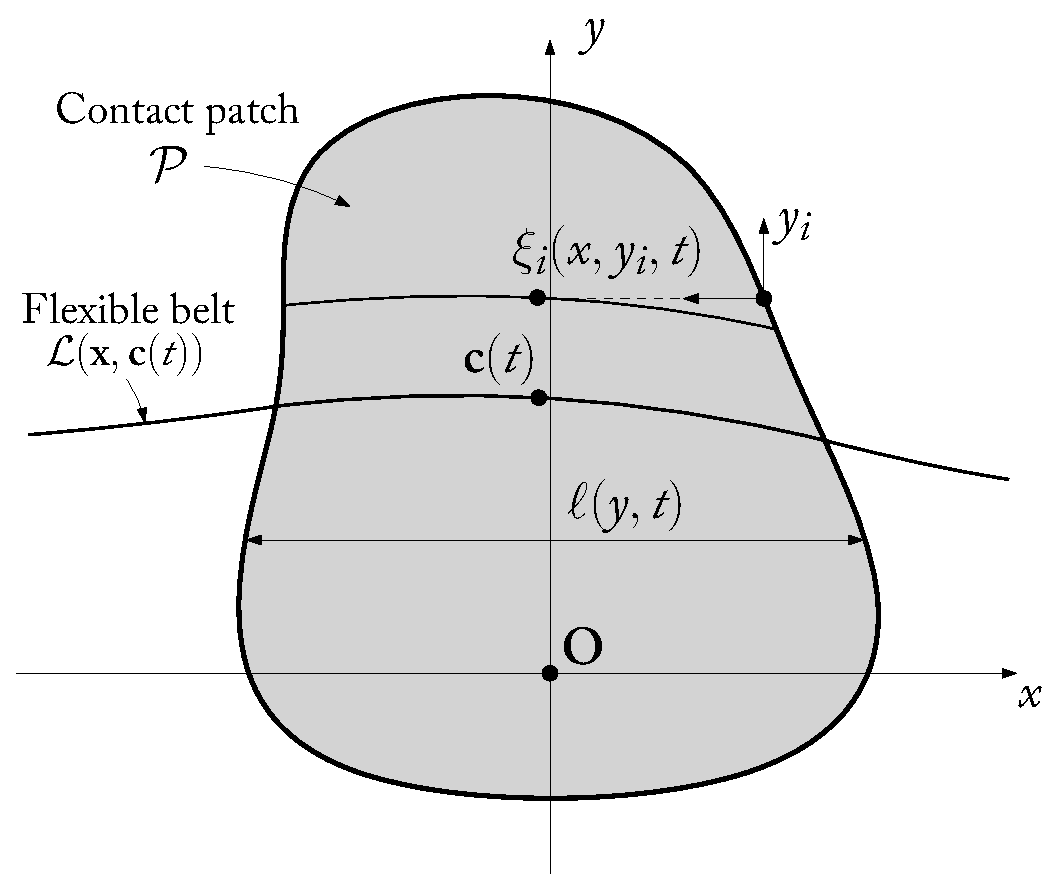
\includegraphics[width=0.9\linewidth]{figures/appendix_3/contact_patch_vertical}
    \caption{Representation of the contact patch region $\sett{P}$ and contact patch reference frame $\bm{\xi}_i(y_i,t)$. Notice that the contact patch is defined as a D-convex and arbitrary region, whose shape is described along the $y$-axis by the quantity $\ell(y,t)$.}
    \label{app3:fig:contact_patch_vertical}
  \end{minipage}
  \hfill
  \begin{minipage}[t]{0.475\linewidth}
    \centering
    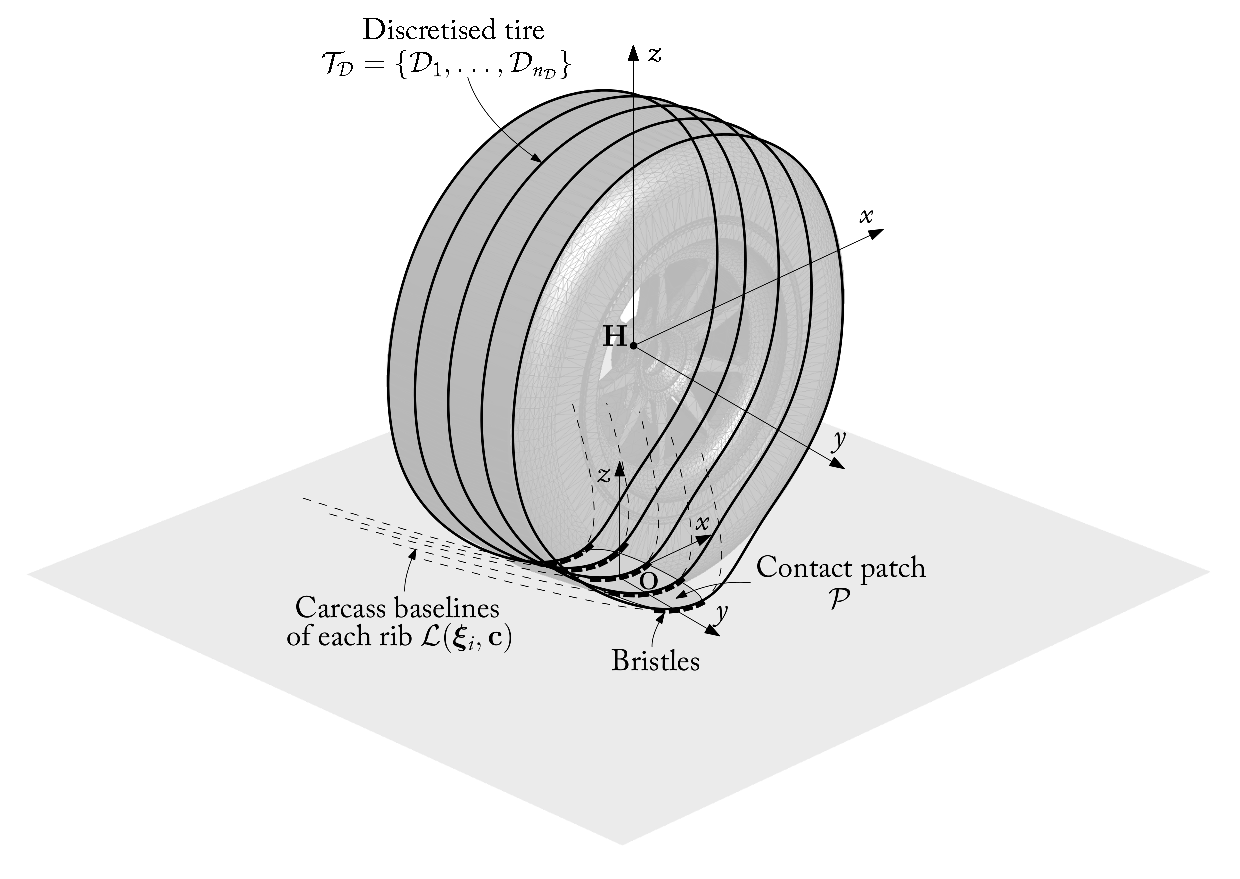
\includegraphics[width=0.9\linewidth, trim={4.35cm 3cm 4.35cm 0cm}, clip]{figures/appendix_3/brush_model}
    \caption{Illustration of the brush model. The tire $\sett{T}$ is discretized into a series of $n_\sett{D}$ ribs. Carcass and bristles are represented as the main components of the model. Conversely, the rim is assumed to be a rigid body and thus has no impact on the tire-road contact.}
    \label{app3:fig:brush_model}
  \end{minipage}
\end{figure}

\subsubsection{Tire-Road Tangential Contact Mechanics Equations}

For each point $\undx{} \in \sett{P}$, given a carcass pose $\vt{c}$, we associate a speed field $\pt{v}(\undx{}, t)$ and a displacement vector $\vt{u}(\undx{}, \vt{c}, t)$. The speed field $\pt{v}$ represents the relative speed between the outer tread layer and the road, while the displacement vector $\vt{u}$ represents the deformation of the material point (also referred to as a \emph{bristle}) located at the coordinate $\undx{}$. Additionally, each material point is also subjected to an external force $\vt{q}(\undx{}, \vt{c}, t)$ generated by the tire-road contact.

We define the generic tangential position as $\undt{} = x\et{e}_x + y\et{e}_y$, the tangential velocity field as $\vt{v}{\undt{}}(\undx{}, \vt{c}, t) = v_x(\undx{}, \vt{c}, t)\et{e}_x + v_y(\undx{},\vt{c},t)\et{e}_y$, the tangential displacement vectors as $\vt{u}{\undt{}}(\undx{},\vt{c},t) = u_x(\undx{},\vt{c},t)\et{e}_x + u_y(\undx{},\vt{c},t)\et{e}_y$, and the tangential stress vector as $vt{q}{\undt{}}(\undx{},\vt{c},t) = q_x(\undx{},\vt{c},t)\et{e}_x + q_y(\undx{},\vt{c},t)\et{e}_y$, in a such a way that
%
\begin{equation}
  \vt{v} =
  \begin{bmatrix}
    \vt{v}{\undt{}} \\
    v_z
  \end{bmatrix} \, text{,} \qquad
  \vt{u} =
  \begin{bmatrix}
    \vt{u}{\undt{}} \\
    u_z
  \end{bmatrix} \, text{,} \qquad \text{and} \qquad
  \vt{q} =
  \begin{bmatrix}
    \vt{q}{\undt{}} \\
    q_z
  \end{bmatrix} \, \text{.}
  \label{app3:eq:ut}
\end{equation}
%
The bristles tangential \emph{micro-sliding speed} is defined as
%
\begin{equation*}
  \vt{v}_s(\undx{},\vt{c},t) =
  \begin{bmatrix}
    v_{sx}(\undx{},\vt{c},t) \\
    v_{sy}(\undx{},\vt{c},t)
  \end{bmatrix} \, \text{,}
\end{equation*}
%
which represents the relative speed between a material point within the contact patch $\sett{P}$ and the road surface $\boundary{R}$. In the following, we will employ an isotropic steady-state Coulomb friction model, which enables us to write the equations governing the contact mechanics between the tire tread layer and the road surface as
%
\begin{equation}
  \vt{v}_s = 0 \iff \|\pt{q}{\undt{}}\| \leq \mu_s q_z
  \qquad \text{and} \qquad
  \vt{q}{\undt{}} = -\mu_d q_z \dfrac{\vt{v}_s}{\|\vt{v}_s\|}
  \iff \vt{v}_s \neq 0 \, \text{.}
  \label{app3:eq:fundamental_eqns}
\end{equation}
%
In these equations, $\mu_s$ represents the static friction coefficient and $\mu_d(\undx{}, \vt{c}, t)$ denotes the ``dynamic'' friction coefficient. It is important to note that~\eqref{app3:eq:fundamental_eqns} is only valid under the assumption of memory-less friction, meaning there is a one-to-one map between the tangential stress and the micro-sliding speed~\cite{canudasdewit2003dynamic}. To solve~\eqref{app3:eq:fundamental_eqns}, two additional sets of equations are necessary. The first set consists of the so-called \emph{tire-road kinematic equations}, which link the wheel hub's relative motion to the deformation field over the contact patch area. The second set includes the \emph{constitutive relations}, which correlate the bristles deformation field to the generated tangential stress $\vt{q}{\undt{}}$.

% % % % % % % % % % % % % % % % % % % % % % % % % % % % % % % % % % % % % % % %

\subsubsection{Rubber Friction}
\label{app3:sec:rubber_friction}

Friction significantly affects tire behavior. As noted in prior works~\cite{selig2014rubber, savkoor1965friction, savkoor1987dry, tiwari2017rubber}, it is influenced by various factors such as tread rubber compound, road surface roughness at both micro and macro levels, relative speed of sliding surfaces, and temperature conditions. To keep the complexity under an acceptable level, we adopt a steady-state Coulomb friction model. In doing so, the dynamic characteristic of friction,  known as \emph{frictional memory}, is disregarded. Such a behavior arises from the fact that the friction coefficient depends not only on the relative sliding speed but also on the contact history, \ie{}, the sliding trajectory~\cite{persson2010rubber}. Including this phenomenon would significantly increase the complexity of the whole tire model, necessitating a dense discretization of the tire tread layer.

Numerous physical formulations aim to capture the relationship between the friction coefficient and sliding speed. One of the most important is the \emph{Savkoor friction law}, which includes the so-called \emph{Stribeck effect}~\cite{savkoor1965friction, savkoor1966some, savkoor1987dry}. When accounting for contact pressure dependency, the ``dynamic'' friction coefficient $\mu_d(\undx{})$ can be expressed as
%
\begin{equation*}
  \mu_d = \mu_w (\mu_{p_0} + \mu_{p_1} \exp( -\mu_{p_2} q_z )) (\mu_k + (\mu_s - \mu_k)) \exp\left( -\mu_{v_0}^2 \log^2 \left( \dfrac{\|\vt{v}_s\|}{v_\mu} + \mu_{v_1} \exp\left(-\dfrac{\|\vt{v}_s\|}{v_\mu}\right)\right)\right) \, \text{,}
\end{equation*}
%
where
%
\begin{itemize}
  \setlength{\itemsep}{0pt}
  \item $\mu_w$ represents the friction coefficient scaling factor, used to tune the friction coefficient under different conditions, such as wet, dry, icy, etc.;
  \item $\mu_s$ is the static friction coefficient;
  \item $\mu_k$ is the kinetic friction coefficient;
  \item $\mu_{p_0}$, $\mu_{p_1}$, $\mu_{p_2}$ are parameters aimed at fitting the rubber-asphalt contact friction pressure dependency;
  \item $\mu_{v_0}$ and $\mu_{v_1}$ are parameters used to reproduce the rubber-asphalt contact friction velocity dependency;
  \item $v_\mu$ is the Stribeck velocity.
\end{itemize}

% % % % % % % % % % % % % % % % % % % % % % % % % % % % % % % % % % % % % % % %

\subsubsection{Tire-Road Kinematic Equations}
\label{app3:sec:kinematic_equations}

The relative velocity between the bristles and the road, first introduced with the name of micro-sliding velocity $\vt{v}_s$, are expressed in Eulerian form similar to that in~\cite{romano2019novel, romano2020unsteadystate, romano2022brush, romano2022analytical, pacejka2012tire, guiggiani2014science, limebeer2018dynamics}. Hence, using~\eqref{app3:eq:parabola} and~\eqref{app3:eq:ut}, $\vt{v}_s$ can be written as
%
\begin{equation}
  \vt{v}_s = V_r\left(\bm{\sigma} + \varphi\et{e}_z \times \left(\sett{L} + \undt{}\right) + \dfrac{\mathrm{d}}{\mathrm{d}x}\sett{L}\,\right) + \dfrac{\mathrm{d}}{\mathrm{d}t}\vt{u}{\undt{}} \, \text{,}
  \label{app3:eq:v_s}
\end{equation}
%
where the material point deformation $\vt{u}{\undt{}}$ is assumed to be small. For a comprehensive description and derivation of such sliding refer to~\cite{rill2020road, pacejka2012tire, guiggiani2014science, limebeer2018dynamics, romano2019novel, romano2022brush, romano2022analytical}. The \emph{theoretical translational slips} $\bm{\sigma}$ represent the normalized difference between the longitudinal and lateral components of the speed of the wheel hub and that of the tire periphery $V_r(y,t) = \omega(t)R_r(y,t)$. Therefore, they are defined as
%
\begin{equation*}
  \bm{\sigma}(y,t) =
  \begin{bmatrix}
    \sigma_x(y,t) \\[0.2em]
    \sigma_y(y,t)
  \end{bmatrix}
  = -\dfrac{1}{|V_r(y,t)|}
  \begin{bmatrix}
    V_x(t) - V_r(y,t) + \dot{x}_c(t) \\[0.2em]
    V_y(t) - R_z(t)\dot{\gamma}(t) + \dot{y}_c(t)
  \end{bmatrix} \, \text{,}
\end{equation*}
%
where $\sigma_x$ and $\sigma_y$ are referred to as the \emph{longitudinal} and the \emph{lateral theoretical slips}. The \emph{theoretical spin slip} $\varphi$ is obtained from
%
\begin{equation*}
  \varphi(y,t) = -\dfrac{\dot{\psi}(t) + \omega(t)\sin(\gamma(t)) + \dot{\theta}_c(t)}{|V_r(y,t)|} \, \text{.}
\end{equation*}
%
The quantity $R_r$ represents the so-called \emph{real rolling radius}, which is calculated as
%
\begin{equation*}
  R_r(y,t) = R(y) - \dfrac{\varrho(y,t)}{3} \, \text{.}
\end{equation*}
%
Other definitions of slips are available in the literature, such as the \emph{practical longitudinal slip} $\kappa$ and \emph{slip angle} $\alpha$~\cite{pacejka2012tire}, which are defined as
%
\begin{equation*}
  \begin{bmatrix}
    \kappa(y,t) \\[0.2em]
    \alpha(y,t)
  \end{bmatrix}
  =
  -\dfrac{1}{|V_x(t)|}
  \begin{bmatrix}
    V_x(t) - V_r(y,t) + \dot{x}_c(t) \\[0.2em]
    \arctan{V_y(t) - R_z(t)\dot{\gamma}(t) + \dot{y}_c(t)}
  \end{bmatrix} \, \text{,}
\end{equation*}
%
and thus
%
\begin{equation*}
  \begin{bmatrix}
    \sigma_x \\[0.2em]
    \sigma_y
  \end{bmatrix}
  =
  \dfrac{1}{1 + |\kappa|}
  \begin{bmatrix}
    \kappa \\[0.2em]
    -\tan(\alpha)
  \end{bmatrix} \, \text{.}
\end{equation*}

Since we are using the same Eulerian form of~\cite{romano2022analytical}, the total time derivative is given by
%
\begin{equation*}
  \dfrac{\mathrm{d}}{\mathrm{d}t} =  \dfrac{\partial}{\partial t} + \vt{v}{\undt{}} \cdot\nabla{\undt{}} \, \text{,}
\end{equation*}
%
where $\nabla{\undt{}}$ collects the tangential components of the gradient, and $\partial/\partial t = 0$ since we are neglecting the viscous component of the Kelvin-Voigt element representing the rubber material point~\cite{meyers2008mechanical}. Neglecting the viscous effect of the tread rubber material eliminates any explicit time dependence in the formulation of brush model forces and torques. Consequently, the tread rubber always operates under stationary conditions. Considering these points, the total derivative of the material point can be explicitly expressed as
%
\begin{equation*}
  \dfrac{\mathrm{d}}{\mathrm{d}t}\vt{u}{\undt{}} = \underbrace{\dfrac{\partial}{\partial t}\vt{u}{\undt{}}}_{=0} + \vt{v}{\undt{}}\cdot\nabla{\undt{}}\vt{u}{\undt{}} \, \text{,}
\end{equation*}
%
where the tangential gradient is given by $\nabla{\undt{}} = [\partial/\partial x, \partial/\partial y]^\top$. The velocity field $\vt{v}{\undt{}}$ of the tread rubber is formulated as
%
\begin{equation*}
  \vt{v}{\undt{}} = -V_r \dfrac{\dfrac{\mathrm{d}}{\mathrm{d}x} \sett{L}}{\Big\|\dfrac{\mathrm{d}}{\mathrm{d}x} \sett{L}\,\Big\|} \, \text{.}
\end{equation*}
%
Given the assumption of small carcass deformations (approximatively $|x_c| < \rho_b$, $|y_c| < \rho_b$, and $|\theta_c| < \pi/10$) and small tire camber angles ($|\gamma(t)| < \pi/10$) the following relationships holds~\cite{romano2022advanced}
%
\begin{equation*}
  \dfrac{\mathrm{d}}{\mathrm{d}x} \sett{L}_x \approx 1 \qquad \text{and} \qquad \dfrac{\mathrm{d}}{\mathrm{d}x} \sett{L}_y \approx 0 \, \text{.}
\end{equation*}
%
The trajectories of the bristles moving within the contact patch are straightened in the longitudinal direction. Therefore, the formulation is constrained to a velocity field of the form $\vt{v}{\undt{}} = [-V_r, 0]^\top$

By separating the longitudinal and tangential displacements of the bristles, we derive the bristle micro-sliding speed formulated as
%
\begin{equation}
  \vt{v}_s = V_r\left( \vt{\bm{\sigma}} + \varphi\huvec_z \times \left(\sett{L} + \undt{}\right) + \dfrac{\mathrm{d}}{\mathrm{d}x}\sett{L} - \dfrac{\mathrm{d}}{\mathrm{d}x}\vt{u}{\undt{}} \right) \, \text{.}
  \label{app3:eq:v_s_int}
\end{equation}

% - - - - - - - - - - - - - - - - - - - - - - - - - - - - - - - - - - - - - - -

\subsubsection{Constitutive Relations}
\label{app3:sec:constitutive_relations}

In the present work, we assume that -- from a frictional perspective -- two regions are identified along the contact patch region \cp{}. The first is the adhesion region \adh{}, where bristle tips do not slide with respect to the ground, generating the so-called adhesive forces. The second is the sliding region \sli{}, where bristles tips slide on the ground surface, producing instead the sliding forces. The boundary separating these two regions is called transition line $\xi_s(\bm{\xi},\vt{c},t)$. Although this assumption may be not realistic in the case of high spin slip value, it greatly simplifies the problem~\cite{romano2022advanced}. By adopting this approach, the domain corresponds to the contact patch interior \interior{P}, where the partial differential equations ruling the tire-road kinematics are defined, and the corresponding \acp{BC} can be uniquely formulated on \boundary{P}~\cite{romano2022analytical}. This research aims to develop a formulation that strikes a balance between realism and computational efficiency, rather than striving for a rigorous closed-form expression for the tangential bristle contact mechanics.

\paragraph{Adhesion Region}

Each individual, material point, acting independently of others,  enters the contact patch through the leading edge in an undeformed state.  As a result of van der Waals molecular bonding and rubber indentation at the rubber/ground interface, the tip of the bristles sticks to the ground. However, due to the micro-sliding velocity $\vt{v}_s$ between the root of the bristles and the road, a tangential deflection $\vt{u}{\undt{}}$ starts to build up, along with tangential stress $\vt{q}{\undt{}}$. Initially null, this bristle deformation increases gradually along the contact length until it reaches the transition line $\xi_s(\bm{\xi},\vt{c})$. This transition line represents the contact length coordinate at which the local force exerted by the bristle deformation in adhesion equals the maximum possible static friction force.

It is important to note that within the adhesion region, the tips of the bristles do not slide relative to the ground, resulting in a zero micro-sliding velocity. Consequently, the deformation of the bristles increases along the contact length direction with a spatial derivative equal to
%
\begin{equation}
  \dfrac{\mathrm{d}}{\mathrm{d}x}\vt{u}{\undt{}} =
  \dfrac{\mathrm{d}}{\mathrm{d}x}
  \begin{bmatrix}
    u_x \\[0.2em]
    u_y
  \end{bmatrix} \, \text{,}
  \label{app3:eq:u_dx}
\end{equation}
%
which is easily found from~\eqref{app3:eq:v_s_int} by imposing $\vt{v}_s = 0$.

We now introduce a new contact patch coordinate system (also depicted in \figurename~\ref{app3:fig:contact_patch_vertical})
%
\begin{equation*}
  \bm{\xi}(y,t) =
  \begin{bmatrix}
    \xi(x,y,t) \\[0.2em]
    \eta \\[0.2em]
    \zeta
  \end{bmatrix}
  =
  \begin{bmatrix}
    \ell(y,t)/2-x \\[0.2em]
    y \\[0.2em]
    z
  \end{bmatrix} \, \text{.}
\end{equation*}
%
The variable $\xi$ represents the distance from the entrance to the longitudinal coordinate, measured longitudinally from the contact patch leading edge. From now on, we will use the superscript ``$\,\bm{\xi}\,$'' to denote variables described in reference system $\bm{\xi}$, \eg{}, $\vt{u}{\undt{}}(\bm{\xi},\vt{c})$. Substituting $\bm{\xi}$ in~\eqref{app3:eq:u_dx} we obtain
%
\begin{equation}
  \dfrac{\mathrm{d}}{\mathrm{d}\xi}\vt{u}{\undt{}}^{\bm{\xi}} =
  \dfrac{\mathrm{d}}{\mathrm{d}\xi}
  \begin{bmatrix}
    u_{x}^{\bm{\xi}} \\[0.2em]
    u_{y}^{\bm{\xi}}
  \end{bmatrix} \, \text{.}
  \label{app3:eq:u_dxi}
\end{equation}
%
The specific deformation $\vt{u}{\undt{}}^{\bm{\xi}}$ at a contact length coordinate $\xi$ and lateral coordinate $y$ is obtained from integrating~\eqref{app3:eq:u_dxi} over space, while imposing the boundary condition $\vt{u}{\undt{}}(\undx{} = [0,y,0]^\top,\vt{c}) = 0$, namely
%
\begin{equation}
  \vt{u}{\undt{}}^{\bm{\xi}} = \int_0^\xi \dfrac{\mathrm{d}}{\mathrm{d}\zeta}\vt{u}{\undt{}}(\zeta,\vt{c}) \,\mathrm{d}\zeta.
  \label{app3:eq:u_xi}
\end{equation}
%
The infinitesimal adherence force at a specific contact length coordinate $\xi$ is determined by the product between~\eqref{app3:eq:u_xi} and the tread tangential stiffness matrix $\pt{k}$
%
\begin{equation*}
  \vt{q}{\undt{}}^{\bm{\xi}} = -\nu\pt{K}{\undt{}}\vt{u}{\undt{}}^{\bm{\xi}} \, \text{.}
\end{equation*}
%
Here, $\nu$ represents the tread pattern void ratio, and $\pt{K}{\undt{}}$ denotes the tangential stiffness matrix. This latter is typically expressed as
%
\begin{equation*}
  \pt{K}{\undt{}} =
  \begin{bmatrix}
    k_{xx} & k_{yx} \\[0.2em]
    k_{yx} & k_{yy}
  \end{bmatrix} \, \text{,}
\end{equation*}
%
where $k_{xy} \approx k_{yx} \ll k_{xx} \approx k_{yy}$, as proofed by \citet{okonieski2003simpified}. The total bristles force induced by the deformation in adherence is obtained by integrating the following over the entire adhesion region \adh{}
%
\begin{equation}
  \vt{F}_a(\vt{c},t) = \int_{\adh} \vt{q}{\undt{}}^{\bm{\xi}} \mathrm{d}\bm{\xi} \, \text{.}
  \label{app3:eq:F_a}
\end{equation}

In the original brush model presented in~\cite{pacejka2012tire}, the self-aligning moment is attributed solely to the asymmetrical distribution of lateral shear stress along the contact length. However, in this study, we will also consider that the difference in longitudinal force on each side of the contact patch contributes to the generation of the self-aligning moment. Thereby, the adhesive self-aligning moment is defined as the cross-product between forces induced by deformation and the position vector (the sum of bristle position and carcass baseline position vectors), which reads
%
\begin{equation}
  \vt{M}_{a}(\vt{c},t) = \int_{\adh} \vt{q}{\undt{}}^{\bm{\xi}} \times \left(\sett{L}^{\bm{\xi}} + \bm{\xi}\right) \mathrm{d}\bm{\xi} \, \text{.}
  \label{app3:eq:M_a}
\end{equation}

\paragraph{Slide Region}

When the local force induced by bristle deformation in adhesion is greater than the local maximum explicable static friction force, the bristle tips begin to slide over the ground with a micro-sliding velocity $\vt{v}_s^{\bm{\xi}} \neq 0$. The local force exerted by bristle deformation in sliding opposes the micro-sliding velocity. Thus, its direction is denoted as
%
\begin{equation*}
  \vt{d}_{\undt{}}(\bm{\xi},\vt{c}) =
  \begin{bmatrix}
    d_{tx}(\bm{\xi},\vt{c}) \\[0.2em]
    d_{ty}(\bm{\xi},\vt{c})
  \end{bmatrix} = -\dfrac{\vt{v}_s^{\bm{\xi}}}{\|{\vt{v}_s^{\bm{\xi}}}\|} \, \text{.}
\end{equation*}
%
The total bristles force induced by the deformation in sliding is determined by integrating the following expression over the entire sliding region \sli{}
%
\begin{equation}
  \vt{F}_s(\vt{c},t) = \int_{\sli} \mu_d^{\bm{\xi}}\,q_z^{\bm{\xi}}\,\vt{d}{\undt{}}^{\bm{\xi}} \, \mathrm{d}\bm{\xi} \, \text{.}
  \label{app3:eq:F_s}
\end{equation}
%
Similar to the adhesive scenario, the self-aligning moment is defined as the cross-product between the local force induced by the sliding and the position vector
%
\begin{equation}
  \vt{M}_s(\vt{c},t) = \int_{\sli} \mu_d^{\bm{\xi}}\,q_z^{\bm{\xi}}\,\vt{d}{\undt{}}^{\bm{\xi}} \times \left(\sett{L}^{\bm{\xi}} + \bm{\xi}\right) \mathrm{d}\bm{\xi} \, \text{.}
  \label{app3:eq:M_s}
\end{equation}

% % % % % % % % % % % % % % % % % % % % % % % % % % % % % % % % % % % % % % % %

\section{A Numerical Solution Approach}
\label{app3:sec:numerical_solution}

Due to the complexity of the problem outlined in the preceding sections, finding an analytical solution is not feasible. Therefore, we need to further analyze the contact zone between the tire and the road and set some more assumptions that will allow us to obtain an effective numerical scheme.

\subsection{Tire-Road Contact Discretization}

An essential characteristic of the contact patch set $\sett{P}$ is its constant compactness and D-convexity along the $\et{e}x$ direction~~\cite{romano2022analytical, matouvsek2001directional}. Leveraging the D-convexity properties enables us to discretize the contact patch into longitudinal sections. To optimize the intersection of the tire and road sets, we discretized the tire set $\sett{T}$ into a series of $n_\sett{D}$ ribs, similarly to the approach in~\cite{chollet2012model, stocco2024novel}. Each tire rib, denoted as $\sett{D}$, is characterized as a conical frustum which is located in $\pt{o}= [0, y_\sett{D}, 0]^\top$ in the $\pt{H}xyz$ coordinate system, with a radius of $R(y_\sett{D})$ and a width of $w_\sett{D}$
%
\begin{equation*}
  \sett{D} = \left\{ w_\sett{D}, y_\sett{D} \in \mathbb{R}, \pt{x} = \left[ x, y, z \right]^\top \in \mathbb{R}^3 ~|~ \sqrt{x^2+z^2} \leq R(y_\sett{D}), |y-y_\sett{D}| \leq \dfrac{w_\sett{D}}{2} \right\} \, \text{.}
\end{equation*}
%
This new representation allows us to build the discretized tire set $\sett{T}_\sett{D}$ as
%
\begin{equation*}
  \sett{T}_\sett{D} = \left\{ \sett{D}_1, \sett{D}_2, \dots, \sett{D}_{n_\sett{D}-1}, \sett{D}_{n_\sett{D}} \right\} \, \text{.}
\end{equation*}
%
Notice that we will employ a set of contact patch coordinate systems $\bm{\xi}_i$ equal to the ribs $n_\sett{D}$. These coordinate systems are redefined as
%
\begin{equation*}
  \bm{\xi}_i(x, y_i, t) =
  \begin{bmatrix}
    \xi_i(x, y_i, t) \\
    \eta_i \\
    \zeta
  \end{bmatrix}
  =
  \begin{bmatrix}
    \ell(y_i, t)/2 - x \\
    y_i \\
    z_i(x)
  \end{bmatrix} \, \text{,}
\end{equation*}
%
where $z_i(x)$ represents the height of the rib $i$ at the point $x$, considering the possibility of the contact patch being sloped in the longitudinal direction. Similar to our previous approach, the variables described in the reference system $\bm{\xi}_i$ will be denoted with the superscript ``$\,\bm{\xi}_{i}\,$'', \eg{}, $\vt{u}_{\pt{t}}(\bm{\xi}_{i}, \vt{c})$. It is worth noting that this tire representation is fully adjustable in scale, allowing for the density of ribs representing the tire to be tailored based on the required accuracy and computational speed for a specific simulation.

By applying the considerations and assumptions outlined in Section~\ref{app3:sec:constitutive_relations} to the constitutive relations, we can express the integrals of forces and moments relative to the adhesion and sliding zones as summations of the components from each rib. Specifically, if the transition coordinate $\xi_s^i$ is assumed to be known, the integrals~\eqref{app3:eq:F_a} and \eqref{app3:eq:M_a} can be analytically solved. Conversely, integrals~\eqref{app3:eq:F_s} and \eqref{app3:eq:M_s} must be numerically calculated.

\subsection{The Transition Coordinate}

Starting from the beginning of each rib contact region, the bristle tips stick to the ground up to the transition coordinate $\xi_s^i$. Determining $\xi_s^i$ entails locating the precise point where the local force induced by bristle deformation in adhesion equals the local maximum static friction force that can be sustained. This requires applying the adhesion criteria outlined in~\eqref{app3:eq:fundamental_eqns}
%
\begin{equation}
  \left(q_{x}^{\bm{\xi}i}\right)^{2} + \left(q_{y}^{\bm{\xi}i}\right)^{2} = \left(\mu_s q_{z}^{\bm{\xi}i}\right)^{2} \, \text{.}
  \label{app3:eq:transition}
\end{equation}

Due to the complexity of the pressure distribution model and the shear field description, finding an analytical solution to equation~\eqref{app3:eq:transition} is not feasible. However, through calculus, it can be demonstrated that the longitudinal and lateral tangential stresses $q_{x}^{\bm{\xi}i}$, $q_{y}^{\bm{\xi}i}$, and normal stress $q_{z}^{\bm{\xi}i}$ can be described by polynomial functions. Consequently, both the right- and left-hand sides of~\eqref{app3:eq:transition} are also polynomials. We can therefore exploit many powerful and robust root-finding algorithms, like Sturm's sequence and the Bisection methods~\cite{bulirsch2002introduction} or the Algorithm 748 by~\citet{alefeld1995algorithm}.

\subsection{Tire Nonlinear System and Solution Method}

To solve~\eqref{app3:eq:nls}, an efficient iterative approach satisfying real-time constraints is necessary. Many tire models, such as those in~\cite{gruber2012normalI, gruber2012normalII, miyashita2010tire, miyashita2003analytical, miyashita2006new, kabe2006new, miyashita2015study}, employ Picard's Iteration Method (also known as the Fixed-Point Method), which is simple to implement but suffers from a slow convergence rate, potentially compromising model robustness. Alternatively, \TaMeTire{} employs a mixed Newton/quasi-Newton iterative method~\cite{fevrier2013method}. If the Jacobian $\vt{J}_\pt{G}$\footnote{$\vt{J}_\pt{G}(\vt{c}) = \partial\vt{G}(\vt{c})/\partial\vt{c}$.} is unavailable, \emph{quasi-Newton} methods can be utilized, albeit with a slight decrease in convergence rate and robustness. Notice that the Frobenius norm\footnote{For a matrix $\pt{A}\in\mathbb{R}^{n \times m}$, the Frobenius norm is defined as $\|\pt{A}\|_\mathrm{F}=\sqrt{\sum_{ij}A_{ij}^2}$.} of the Jacobian $\vt{J}_\pt{F}$\footnote{$\vt{J}_\pt{F}(\vt{c}) = \partial\vt{F}(\vt{c})/\partial\vt{c}$.} is typically small ($\|\vt{J}_\pt{F}\|_\mathrm{F} \ll 1$), while the Frobenius norm of the carcass stiffness matrix Jacbobian $\vt{J}_\pt{K}$ is usually large ($\|\vt{J}_\pt{K}\|_\mathrm{F} \gg 1$). Therefore, a good first approximation of $\vt{J}_\pt{G}$ is given by
%
\begin{equation*}
  \vt{J}_\pt{G} = \vt{J}_\pt{K} - \vt{J}_\pt{F} \approx \vt{J}_\pt{K} \, \text{.}
\end{equation*}
%
If we set the initial iteration point at $\vt{c} = [0,0,0]^\top$, the bottoming effect of the carcass stiffness is absent. As a consequence, the initial estimation of the Jacobian $\vt{J}_\pt{G}$ can be straightforwardly computed by accounting solely for the structural and inflation pressure components of the carcass stiffness.

% % % % % % % % % % % % % % % % % % % % % % % % % % % % % % % % % % % % % % % %

\section{Numerical Performance and Validation}
\label{app3:sec:numerical_experiments}

In this section, we present numerical simulations to validate the tire model and the numerical solution approach. Specifically, we will compare the performance of the quasi-Newton methods used to solve the non-linear system of equations~\eqref{app3:eq:nls}, as well as the fitting quality of the tire model to experimental data. A comparison with the \MagicFormulae{} is also provided.

\subsection{Performance of the Quasi-Newton Methods}

We evaluate the performance of the quasi-Newton numerical methods mentioned earlier. Specifically, we aim to identify the most suitable method for solving the non-linear system of equations~\eqref{app3:eq:nls} among Picard Iteration Method (PIM), Greenstadt's $1^\text{st}$ Method (G1M)~\cite{spedicato1978some}, Greenstadt's $2^\text{nd}$ Method (G2M)~\cite{spedicato1978some}, Eirola-Nevanlinna Method (ENM)~\cite{eirola1989accelerating}, Broyden's Bad Method (BBM)~\cite{broyden1965class},
Broyden's Good Method (BGM)~\cite{broyden1965class}, Broyden's Combined Method (BCM)~\cite{martinez1982sobre}, and their respective dumped versions, denoted with the prefix ``D-''. We will compare these algorithms based on function evaluations, iterations, convergence speed, and success ratio. Table~\ref{app3:tab:timing} presents the performance data of the quasi-Newton solvers. The tests are conducted on a set of $10^5$ simulations with inputs distributed evenly within the following ranges $\sigma_x\in[-1,1]$, $\sigma_y\in[-1,1]$, $\varphi\in[-0.1,0.1]$, $F_z\in[0,5\cdot10^5]$, and $\gamma \in [-\pi/10, \pi/10]$, which represent typical operating conditions for a passenger car tire. All tests are performed on a shielded CPU. The simulation platform is a Concurrent\textsuperscript{\textregistered} iHawk\textsuperscript{\texttrademark} with \SI{2.5}{\giga\hertz} Intel\textsuperscript{\textregistered} Xeon\textsuperscript{\textregistered} Silver 4215 8-core, \SI{11}{\mega\byte} cache, \SI{32}{\giga\byte} DDR4 \ac{RAM}, and \SI{64}{\bit} RedHawk\textsuperscript{\texttrademark} Linux real-time operative system with CentOS distribution.

As depicted in Table~\ref{app3:tab:timing}, both the PIM and D-PIM fail to converge to the solution with the required tolerance. The G1M and D-G1M can not complete the tests due to overflow issues. Conversely, the G2M and ENM, and their dumped version, D-G2M and D-ENM, show a good success ratio but exhibited high average and variance iterations and function evaluations. Although the pure BBM suffered from overflow issues, its dumped version, D-BBM, successfully converged to the solution with the required tolerance and maintained an acceptable success ratio. The BGM and BCM, as well as their dumped versions, D-BGM and D-BCM, demonstrated the best performance overall. They exhibited the highest success ratio and the lowest average and variance in both iterations and function evaluations. Notably, the BCM showed superior computational efficiency. It is worth mentioning that no relaxation steps were accepted in D-BCM. Consequently, the performance of the BCM method is deemed excellent for meeting the demands of hard real-time simulations, \ie{}, achieving a computational time of less than \SI{1}{\milli\second}. Only a small percentage of the tests required and a high number of iterations, however, in these cases the vertical load and resulting carcass deformations exceeded the structural limits, leading to instability in the iterative process.

The bottom part of Table~\ref{app3:tab:timing} presents the performance of the BCM in relation to the number of ribs. Notably, the number of ribs does not impact the efficacy of the iterative method but merely affects the computational time. This arises from the fact that a change in the number of ribs does not alter the number of unknowns in~\eqref{app3:eq:nls}. Consequently, the computational time scales linearly with the number of ribs. However, it is worth noting that the variance of the computational time increases more than linearly due to small yet significant variations in the performance of Algorithm 748.

\begin{table}[htb]
  \centering
  \caption{Comparison between quasi-Newton methods' performance based on a dataset comprising $10^5$ tests. The inputs are evenly distributed within the ranges $\sigma_x \in [-1, 1]$, $\sigma_y \in [-1, 1]$, $\varphi \in [-0.1, 0.1]$, $F_z \in [0, 5\cdot10^5]$, and $\gamma \in [-\pi/10, \pi/10]$, using a 325/660R13 race car tire discretized with $5$ ribs. Convergence is considered achieved when $\|\pt{G}(\vt{c})\|_2 \le 10^{-8}$ and $\|\vt{c}_{k+1} - \vt{c}_{k}\|_2 \le 10^{-16}$. Maximum algorithm iteration and relaxation steps are set to 100 and 10, respectively. The bottom part of the table demonstrates the impact of changing the number of ribs on the BCM method's performance. \\
  \emph{Symbols legend}: \mini{} minimum number of evaluations/iterations, \maxi{} maximum number of evaluations/iterations, \meai{} average evaluations/iterations, \vari{} evaluations/iterations variance.
  }
  \label{app3:tab:timing}
  \small
  {\footnotesize\begin{tabularx}{0.75\textwidth}{*{6}{Y}}%{\textwidth}{*{14}{Y}}
  %\multicolumn{14}{c}{\textbf{Quasi-Newton Methods Performance with 5 Ribs}} \\
  \multicolumn{6}{c}{\textbf{Quasi-Newton Methods Performance with 5 Ribs}} \\
  \toprule
  \multirow{2.25}{*}{\textbf{Method}} &
  %\multicolumn{4}{c}{\textbf{Evaluations} ($-$)} &
  %\multicolumn{4}{c}{\textbf{Iterations} ($-$)} &
  \multicolumn{4}{c}{\textbf{Time} (\USI{\micro\second})} &
  \multirow{2}{*}{\textbf{Success}} \\
  \cmidrule(l{4pt}r{4pt}){2-5}
  %\cmidrule(l{4pt}r{4pt}){6-9}
  %\cmidrule(l{4pt}r{4pt}){10-13}
  %& \mini{} & \maxi{} & \meai{} & \vari{} & \mini{} & \maxi{} & \meai{} & \vari{}
    & \mini{} & \maxi{} & \meai{} & \vari{} & \\
  \midrule
  PIM   %& $100$ & $100$ & $100.0$ & $0.00$    & $100$ & $100$ & $100.0$ & $0.0$
    & $518.0$ & $7949.0$ & $617.2$  & $13953.2$  & $0.0\%$   \\ \hline
  G1M   %& $-$   & $-$   & $-$     & $-$       & $-$   & $-$   & $-$     & $-$
    & $-$     & $-$      & $-$      & $-$        & Overflow  \\ \hline
  G2M   %& $4$   & $100$ & $9.2$   & $55.8$    & $4$   & $100$ & $9.2$   & $55.8$
    & $23.5$  & $1089.4$ & $69.0$   & $5252.0$   & $99.5\%$  \\ \hline
  ENM   %& $6$   & $200$ & $11.9$  & $234.0$   & $3$   & $100$ & $6.5$   & $58.5$
    & $25.0$  & $2025.0$ & $81.5$   & $11002.8$  & $99.4\%$  \\ \hline
  BBM   %& $-$   & $-$   & $-$     & $-$       & $-$   & $-$   & $-$     & $-$
    & $-$     & $-$      & $-$      & $-$        & $0.0\%$   \\ \hline
  BGM   %& $4$   & $100$ & $8.8$   & $18.4$    & $4$   & $100$ & $8.8$   & $18.4$
    & $22.6$  & $948.1$  & $62.5$   & $1973.0$   & $99.9\%$  \\ \hline
  BCM   %& $4$   & $17$  & $8.4$   & $6.7$     & $4$   & $17$  & $8.4$   & $6.7$
    & $22.9$  & $264.4$  & $55.7$   & $885.9$    & $100.0\%$ \\ \hline
  D-PIM %& $100$ & $496$ & $190.7$ & $13628.1$ & $100$ & $100$ & $100.0$ & $0.0$
    & $507.0$ & $5383.0$ & $1151.9$ & $568491$   & $0.0\%$   \\ \hline
  D-G1M %& $-$   & $-$   & $-$     & $-$       & $-$   & $-$   & $-$     & $-$
    & $-$     & $-$      & $-$      & $-$        & Overflow  \\ \hline
  D-G2M %& $4$   & $376$ & $11.3$  & $572.4$   & $4$   & $100$ & $9.3$   & $57.1$
    & $21.5$  & $3195.5$ & $80.4$   & $40321.9$  & $99.5\%$  \\ \hline
  D-ENM %& $6$   & $513$ & $12.8$  & $829.7$   & $3$   & $100$ & $6.3$   & $44.3$
    & $27.0$  & $5207.7$ & $97.5$   & $52752.6$  & $99.5\%$  \\ \hline
  D-BBM %& $4$   & $125$ & $11.0$  & $58.0$    & $4$   & $42$  & $9.3$   & $12.8$
    & $22.3$  & $1284.0$ & $76.9$   & $5126.3$   & $100.0\%$ \\ \hline
  D-BGM %& $4$   & $376$ & $9.7$   & $110.6$   & $4$   & $100$ & $8.7$   & $15.1$
    & $21.3$  & $3238.9$ & $67.0$   & $8142.9$   & $99.9\%$  \\ \hline
  D-BCM %& $4$   & $35$  & $9.1$   & $14.6$    & $4$   & $17$  & $8.4$   & $6.7$
    & $22.5$  & $316.8$  & $62.1$   & $1615.1$   & $100.0\%$ \\
  \bottomrule
\end{tabularx}%
\vspace*{0.5em}
\begin{tabularx}{0.75\textwidth}{*{6}{Y}}%{\textwidth}{*{14}{Y}}
  %\multicolumn{14}{c}{\textbf{Broyden Combined Method Performance}} \\
  \multicolumn{6}{c}{\textbf{Broyden Combined Method Performance}} \\
  \toprule
  \multirow{2.25}{*}{\textbf{Ribs}} &
  %\multicolumn{4}{c}{\textbf{Evaluations} ($-$)} &
  %\multicolumn{4}{c}{\textbf{Iterations} ($-$)} &
  \multicolumn{4}{c}{\textbf{Time} (\USI{\micro\second})} &
  \multirow{2}{*}{\textbf{Success}} \\
  \cmidrule(l{4pt}r{4pt}){2-5}
  %\cmidrule(l{4pt}r{4pt}){6-9}
  %\cmidrule(l{4pt}r{4pt}){10-13}
  %\multirow{0.5}{*}{\textbf{of Ribs}}
  %& \mini{} & \maxi{} & \meai{} & \vari{} & \mini{} & \maxi{} & \meai{} & \vari{}
    & \mini{} & \maxi{} & \meai{} & \vari{} & \\
  \midrule
  $1$  %& $6$     & $11$    & $7.9$   & $10.3$
       %& $6$     & $11$    & $7.9$   & $10.3$
       & $12.1$  & $89.0$  & $19.4$  & $20.6$  & $100.0\%$ \\ \hline
  $5$  %& $4$     & $17$    & $7.9$   & $10.3$
       %& $4$     & $17$    & $7.9$   & $10.3$
       & $22.9$  & $264.4$ & $55.7$  & $885.9$ & $100.0\%$ \\ \hline
  $10$ %& $6$     & $11$    & $7.9$   & $10.3$
       %& $6$     & $11$    & $7.9$   & $10.3$
       & $106.9$ & $361.8$ & $167.3$ & $1746.22$ & $100.0\%$ \\ \hline
  $15$ %& $6$     & $11$    & $7.9$   & $10.3$
       %& $6$     & $11$    & $7.9$   & $10.3$
       & $158.0$ & $523.5$ & $249.4$ & $3878.2$ & $100.0\%$ \\ \hline
  $20$ %& $6$     & $11$    & $7.9$   & $10.3$
       %& $6$     & $11$    & $7.9$   & $10.3$
       & $210.1$ & $693.3$ & $332.9$ & $7028.7$ & $100.0\%$ \\ \hline
  $25$ %& $6$     & $11$    & $7.9$   & $10.3$
       %& $6$     & $11$    & $7.9$   & $10.3$
       & $262.7$ & $858.4$ & $414.0$ & $10708.3$ & $100.0\%$ \\
  \bottomrule
\end{tabularx}}%
\end{table}

\subsection{Validation of the Tire Model}

To demonstrate the effectiveness of the proposed fitting procedure, we validate the proposed tire model under pure slip conditions by comparing its predictions with those of a \MagicFormulae{}~5.2~\cite{pacejka2012tire} on the fitting of experimental data for a \Hoosier{} 18x6-10 LCO tire. As previously mentioned in the introduction, the dataset is obtained from the Calspan \ac{TIRF} for the \ac{FSAE} \ac{TTC} testing program~\cite{kasprzak2006formula}. In Figure~\ref{app3:fig:fsae_pure}, we compare the fitting of the longitudinal and lateral forces and aligning moment for the \Hoosier{} tire at several discrete values of vertical load with zero camber angle. The results indicate that the proposed model provides data fitting comparable to the \MagicFormulae{}~5.2 for the lateral force, while a higher \ac{RMS} error is observed for the longitudinal force and aligning moment. Given the limited number of parameters and the simplicity of the proposed model, these results are considered satisfactory.

\begin{figure}[htb]
  \centering
  \small{\includetikz{figures/appendix_3/Fx_fsae.tex}}
  \small{\includetikz{figures/appendix_3/Fy_fsae.tex}}
  \small{\includetikz{figures/appendix_3/Mz_fsae.tex}}
  \caption{Comparison between the \MagicFormulae{} and the proposed model regarding the fitting of experimental data for a \Hoosier{} 18x6-10 LCO tire. Experiments are performed under pure longitudinal and lateral slips at several discrete values of vertical load with zero camber angle. The dataset is provided by the Calspan \ac{TIRF} for the \ac{FSAE} \ac{TTC} testing program~\cite{kasprzak2006formula}. \emph{Lines and marks legend}: \textbullet~experimental data, \textbf{---}~proposed model, and \textbf{--~--}~\MagicFormulae{}~5.2. \emph{Colors legend}: \textcolor{mycolor1}{$\blacksquare$}~$F_z = \SI{222}{\newton}$, \textcolor{mycolor2}{$\blacksquare$}~$F_z = \SI{444}{\newton}$, \textcolor{mycolor3}{$\blacksquare$}~$F_z = \SI{667}{\newton}$, \textcolor{mycolor4}{$\blacksquare$}~$F_z = \SI{890}{\newton}$, and \textcolor{mycolor5}{$\blacksquare$}~$F_z = \SI{1120}{\newton}$.}
  \label{app3:fig:fsae_pure}
\end{figure}

% % % % % % % % % % % % % % % % % % % % % % % % % % % % % % % % % % % % % % % %
